\documentclass[a4paper,oneside,article]{memoir}
\usepackage[UTF8]{inputenc}
\usepackage[Danish]{babel}
\usepackage[T1]{fontenc}

\setsecnumdepth{subsection}
\setcounter{tocdepth}{5}
\setcounter{secnumdepth}{4}

\setsecnumdepth{subsection}
\usepackage{lmodern}
\usepackage{parskip}

%Billeder skal
\usepackage{graphicx}
\graphicspath{ {Afsnit/} }
\usepackage{float}
\usepackage{wrapfig}

% Listings og color bruges til at vise vores VHDL kode med.
\usepackage{listings}
\usepackage{color}

\definecolor{dkgreen}{rgb}{0,0.6,0}
\definecolor{gray}{rgb}{0.5,0.5,0.5}
\definecolor{mauve}{rgb}{0.58,0,0.82}

\lstset{frame=tb,
  language=C++,
  aboveskip=3mm,
  belowskip=3mm,
  showstringspaces=false,
  columns=flexible,
  basicstyle={\small\ttfamily},
  numbers=none,
  numberstyle=\tiny\color{gray},
  keywordstyle=\color{blue},
  commentstyle=\color{dkgreen},
  stringstyle=\color{mauve},
  breaklines=true,
  breakatwhitespace=true,
  tabsize=3
}



\title{Detaljerede Sprint beskrivelser 3. Semesterprojekt - Goofy Candy Gun\\ Gruppe 3}

\author{
  Rieder, Kasper\\
  \texttt{201310514}
  \and
  Jensen, Daniel V.\\
  \texttt{201500152}
  \and
  Nielsen, Mikkel\\
  \texttt{201402530}
  \and
  Kjeldgaard, Pernille L.\\
  \texttt{PK94398}
  \and
  Konstmann, Mia\\
  \texttt{201500157}
  \and
  Kloock, Michael\\
  \texttt{201370537}
  \and
  Rasmussen, Tenna\\
  \texttt{201406382}
}

\pagestyle{headings}

\begin{document}
	
	\frontmatter
	\maketitle

	\section{Sprint 1}
	\textbf{19/2/16 - 14/3/16}\newline
	\textbf{Varighed:} 3 uger\newline
	\textbf{Scrum master: }Kasper \newline \newline
	Formålet med det første sprint var at dokumentere, implementere og teste use case 2, Test Kommunikationsprotokoller.
	Sprintet startede ud med at lave en backlog i Pivotal Tracker. Der blev lavet userstories på baggrund af brugerønsker samt userstories til de dokumenter, der udgør de tre færdige rapporter. Herefter blev to userstories udvalgt til sprint backloggen, der skulle arbejdes på i dette sprint. Disse userstories består af underopgaver, der hørte til implementeringen af hardware og software. Når en underopgave blev færdiggjort, blev den krydset af i userstory'en. \newline
	
	I kravspecifikationen blev det bestemt der skulle anvendes tre PSoC til I2C kommunikationen mellem GUI, motor og nunchuck. Under arkitektur dannelsen så vi at PSoC2 forbundet til nunchucken kun pollede for information og videredesendte det. Ved at fjerne PSoC2 forbundet til nunchuck'en og forbinde den til PSoC1 forbundet til motoren. Dermed overtager PSoC1 funktionaliteten af PSoC2 og vi undgår unødig kommunikation. \newline
	
	Under sprintet udførte vi diverse opgaver, der ikke stod i sprint backloggen. Dette blev gjort da vi havde glemt at definere dem som userstories da vi udvalgt opgaver til sprintbackloggen. Dermed er der blevet udført meget mere under sprintet end der kan ses på Pivotal Tracker. \newline
	
	Under dette sprint har vi anvendt logbøger, i stedet for daglig stand up møder. Der blev hver morgen noteret det, som man egentligt ville have nævnt til de daglige møder. Det gav en del arbejde til scrum masteren, der skulle tjekke hver dag om alle havde lavet dagens indlæg. Derudover forsvandt kommunikationen mellem gruppensmedlemmer i perioder, da der ikke var nogen andre end scrum masteren, der kiggede logbøgerne igennem. Dette gav anledning til en del miskommunikation omkring arbejdsdage og arbejdsopgaver. For at undgå dette vil vi forsøge os med daglige stand up møder, med vejlederen, i næste sprint. \newline
	
	\begin{figure}[H]
		\centering
		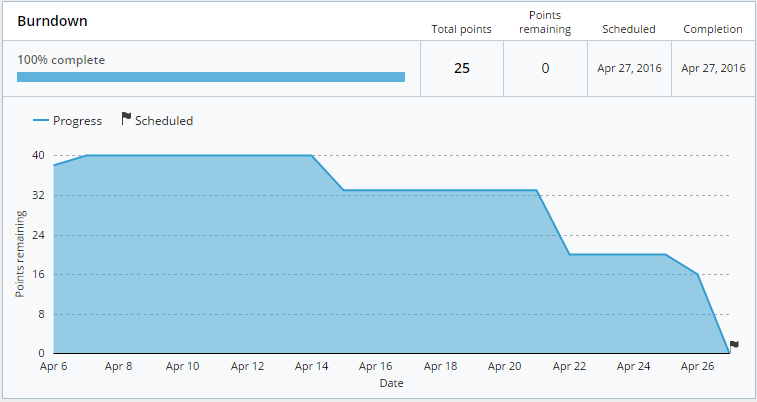
\includegraphics[width=\textwidth]{Projektgennemfoerelse/images/burndown1}
		\caption{Burndown chart for sprint 1}
		\label{ref:Burndown1}
	\end{figure}
	
	På figur \ref{ref:Burndown1} ses et burndown chart for første sprint. Dette billede er taget efter sprintet er afsluttet og derfor ser det ud til at 100\% af opgaverne er færdiggjorte. Ved at se på grafen kan man se at lige  inden sprintet afsluttede manglede der 16 point på sprintbackloggen. Grafen er præget af en plateau effekt. Dette skyldes størrelsen på opgaverne på sprintbackloggen. Det ser ud til at der er inaktive perioder efterfulgt af et dyk. Da vi ikke færdiggjorde nogen af vores userstories til fulde, medførte det at vi tilsyneladende ikke har opnået nogen resultater i dette sprint.  \newline
	
	\textbf{Under dette sprint har vi lært:}
	\begin{itemize}
		\item At user stories skal være mere findelt, for at kunne vise udviklingen af projektet
		\item At strukturen for PSoC opsætningen ikke var hensigtsmæssig, da PSoC1 kunne overtage funktionaliteten af PSoC2
		\item At vi skal holde os til sprint backloggen og kun arbejde på de opgaver vi har defineret for sprintet
		\item At der skal bruges mere tid til at opdatere gruppens status
	\end{itemize}
	
	Da sprintet var færdig er vi gået tilbage og ændret på sprint backloggen for både at findele de userstories vi havde inkluderet og for at dokumentere de ting der er blevet udført i dette sprint, som ikke var inkluderet. Derudover tager den erfaring vi har fået med arkitekturen med til et af de næste sprint hvor use case 2 skal implementeres. Da vi ikke havde så meget erfaring med scrum mistede vi under sprintet overblikket og dermed kom vi for langsomt i gang med implementeringen. Dette skyldes både vores uerfarenhed med scrum og dårlig tidsestimering. Vi opnåede meget i dette sprint, dog opnåede vi ikke det ønskede mål, som var en færdig implementeret use case 2. 
	
	
	
	\section{Sprint 2}
	\textbf{16/3/16 - 6/4/16}\newline
	\textbf{Varighed:} 3 uger\newline	
	\textbf{Scrum master: }Pernille \newline
	Formålet med anden sprint var at designe og implementere software og hardware til use case 2, Test Kommunikationsprotokoller. Sprintet startede ud med sprintplanlægningsmøde. Her blev der i gruppen blev aftalt hvilke userstories skulle laves under sprintet. Da disse var fastlagt blev der aftalt et sprintplanlægningsmøde med vejlederen, der hjalp med tidsestimering af disse opgaver. Dette var en langsommelig process, men dette var nødvendigt da vi ikke havde anvendt Pivotal Tracker ordentligt og havde problemer med tidsestimering i sidste sprint. Under mødet blev opgaverne også prioriteret, noget som ikke blev gjort i sidste sprint, dermed blev der skabt et overblik af de vigtigste opgaver til sprintet. \newline
	
	Som noget nyt forsøgte gruppen sig med stand up meetings. Dette var et forsøg på at anvende scrum i et større omfang end vi tidligere har gjort. I en hel uge blev der afholdt morgen møder med vejlederen inden dagens lektioner. Til disse møder blev der nævnt hvad man ellers ville have været skrevet i logbøgerne. Dette gjorde arbejdet lettere for scrum masteren, da hun skulle fungere som ordstyrer til disse møder, i stedet for at læse logbøger. Møderne gav gruppens medlemmer et overblik som man ikke havde fået ved logbøgerne, da man ikke aktivt skulle opsøge information omkring hvad de andre medlemmer foretog sig. Gruppen oplevede, at fordi vi havde kontakt med vejlederen dagligt, fik vi hurtig respons til opstandne problemer og hjælpen var bedre end det vi kunne modtage fra en mail. Der var dog nogle problemer med møderne, da den uge de kørte over, var en uge hvor der skete meget samarbejde. Dermed blev møderne en samtale omkring hvad hardware- og softwaregruppen havde lavet dagen forinden. Stå op møderne ville have fungeret meget bedre hvis de havde foregået i en uge hvor der blev arbejdet mere individuelt. \newline
	
	En af grundene til at opgaverne fra sprint backloggen ikke var fuldført var fordi at der i midten af dette sprint var påske ferie. Dette gav anledning til diskussioner i gruppen da der ikke var enighed omkring antallet af arbejdstimer i ferien. Løsningen på dette var at der blev aftalt to arbejdsdage i ferien, hvor der skulle arbejdes på projektet. Resten af ferien var det op til hver gruppemedlem at bestemme hvilke dage der skulle arbejdes. \newline
	
	\begin{figure}[H]
		\centering
		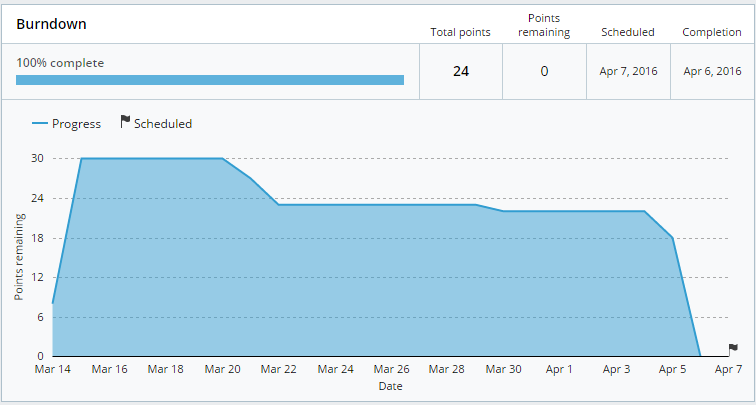
\includegraphics[width=\textwidth]{Projektgennemfoerelse/images/burndown2}
		\caption{Burndown chart for sprint 2}
		\label{ref:Burndown2}
	\end{figure}
	
	På figur \ref{ref:Burndown2} ses anden sprints burndown chart. Her ses at ved sprint afslutningen var der stadig 18 point i ufærdige opgaver på sprintbackloggen. Det ses også at sprintet blev afsluttet en dag tidligere end forventet. Grafen er stadig præget af en plateau effekt. Denne gang er det i en værre grad end ved første sprint. Dette skyldes formenligt flere dages inaktivitet under ferien og problemer med kommunikationsprotokoller i software. \newline 
	
	\textbf{Under dette sprint har vi lært:}
	\begin{itemize}
		\item At give opgaver realistiske tidsestimater
		\item At prioritere opgaver i backloggen
		\item At stå op møder fungerer ikke optimalt når der sker meget samarbejde
		\item At der skal bruges mere indsats for at kommunikere med gruppen 
	\end{itemize}
	
	Under dette sprint havde gruppen mere erfaring med scrum og anvendelsen af Pivotal Tracker end vi havde tidligere. Eftersom gruppen har arbejdet sammen i et længere stykke tid sker der færrer miskommunikationer. Da der stadig er problemer med tidsestimeringen blev backloggen ikke tømt for opgaver, men vi er kommet længere end forrig sprint. Målet for dette sprint er ikke opnået, men der er blevet udført nok til at vi føler at sprintet var vellykket.
	
	\section{Sprint 3}
	\textbf{7/4/16 - 27/4/16}\newline
	\textbf{Varighed: }3 uger \newline
	\textbf{Scrum master: }Mia \newline \newline
	Formålet med tredje sprint var at færdiggøre use case 2, samt få implemeteret dele af hardware til use case 1. Til sprintplanlægningsmødet oplevede gruppen et stort mandefald, da nogle af gruppens medlemmer var syge. Dette hindrede resten af gruppen i at planlægge sprintet efter alles ønsker. Da der var nogle medlemmer, som var dukket op på trods af sygdom, havde et ønske at tage hjem inden dagens lektioner blev dette møde timeboxed til en time. Under denne time fik gruppen fastlagt målet for sprintet og defineret de opgaver der skulle til for at nå dette mål. Da alle gruppens medlemmer ikke var til stede og der var sat den nødvendige tid af til sprintplanlægningsmødet oplevede vi igen at opgaverne ikke var veldefinerede og der var opgaver der manglede på sprint backloggen. \newline
	
	Under dette sprint deltog alle gruppens medlemmer i et scrumkursus som Systematic udbyder. Da scrum er den udviklingsmodel som anvendes til dette projekt, forekom det naturligt for gruppens deltagere at deltage som en gruppe. Hermed kunne de erfaringer og konklusioner som blev draget til kurset blive anvendt til at styrke gruppens kommunikation og samarbejde. 
	Til kurset blev der undervist i omfattende teori omkring scrum, der blev afholdt diskussioner og scrum blev taget i brug gennem øvelser. Øvelserne fokuserede på at træne evner, som har afgørende betydning for scrum. Disse inkluderede tidsestimering, planlægning, kommunikation og organisering. \newline
	
	Kommunikation er afgørende når der arbejdes med scrum. Dette noget vi oplevede da arbejdede med øvelserne til scrumkurset og da vi så på arbejdsgangen på Systematic. Gruppen har indset at logbøgerne, som blev genoptaget efter det fejlede forsøg med fysiske stand up meetings, ikke fungerede i en grad til at de kunne erstatte de fysiske stand up meetings, som scrum kræver. Kommunikationen i gruppen er ikke optimal, da der arbejdes mere individulet end der er blevet gjort hidtil, og der sker ingen kommunikation på tværs af undergrupperne. Derfor oprettes der en Facebook samtale, som skal sørge for kommunikationen. Med dette anvendes en platform som gruppen i forvejen bruger i dagligdagen til at opretholde kommunikationen.  \newline 
	
	\begin{figure}[H]
		\centering
		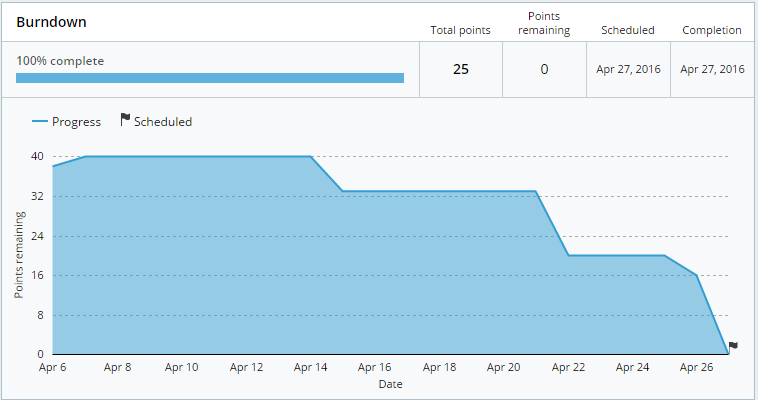
\includegraphics[width=\textwidth]{Projektgennemfoerelse/images/burndown3}
		\caption{Burndown chart for sprint 3}
		\label{ref:Burndown3}
	\end{figure}
	
	På figur \ref{ref:Burndown3} ses burndown chartet for sprint 3. Under dette sprint var opgaverne delt fint op, men det ses i figuren at der stadig er en plateau effekt. Dette skyldes at der var stor afhængighed mellem mange af de små opgaver. Det betød at der skulle meget forarbejde til at løse en opgave, men når denne så var færdiggjort, kunne andre opgaver hurtigt krydses af. Ved sprintafslutning stod vi tilbage med 16 point på backloggen. Dette skyldes at der var lagt op til mange rapportskrivnings opgaver, som var påbegyndt, men vurderet for udfærdig til at blive krydset af. \newline
	
	\textbf{Under dette sprint har vi lært:}
	\begin{itemize}
		\item At der skal sættes den nødevendige tid af til afholde sprintplanlægsningsmødet
		\item Hvordan scrum fungerer i praksis i forbindelse med en arbejdsplads
		\item At der fortsat skal ydes en større indsats for at kommunikere i gruppen
	\end{itemize}
	
	Under dette sprint opnåede gruppen sit sprintmål, som var færdiggørelse af use case 2. Alt software og hardware, der skal til, for at kunne udføre use case 2 er færdig implementeret og implementation for dele af hardware til use case 1 er påbegyndt. I dette sprint fik gruppen mulighed for at arbejde intensivt med scrum og kunne tage disse erfaringer med til selve projektet. 
	
	\section{Sprint 4}
	\textbf{27/4/16 - 18/5/16}\newline
	\textbf{Varighed: }3 uger \newline
	\textbf{Scrum master: }Tenna \newline \newline
	Formålet med fjerde og sidste sprint var at afslutte alle påbegyndte implementationsopgaver og starte på rapportskrivning. Da sprintbackloggen tidligere har været præget af problemer med tidsestimering skete der en taktik ændring til sprintplanlægningsmødet. Der blev set på hvor mange timer der var til rådighed for projektarbejde og lagde alle mandetimerne sammen. Herefter definerede vi time antallene for store, mellem og små opgaver, henholdsvis over 12 timer, 12 timer og 4 timer. Herefter blev der sat opgaver på sprintbackloggen indtil alle mandetimerne var afsat på disse opgaver. Dette resulterede i det største antal point på sprintbackloggen, i forhold til de forgående sprint.
	
	\begin{figure}[H]
		\centering
		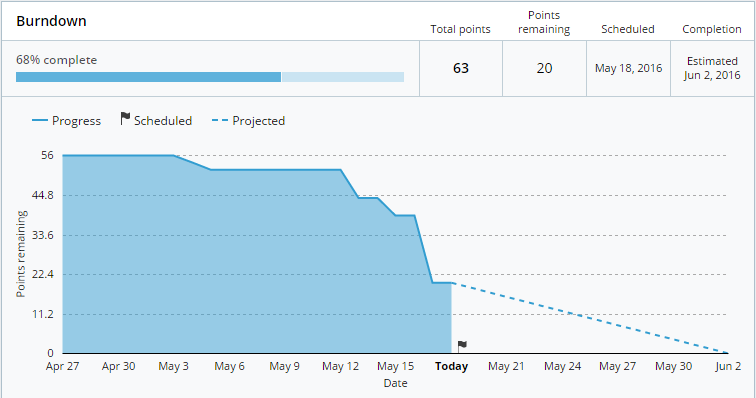
\includegraphics[width=\textwidth]{Projektgennemfoerelse/images/burndown4}
		\caption{Burndown chart for sprint 4}
		\label{ref:Burndown4}
	\end{figure}
	
	På figur \ref{ref:Burndown4} ses et burndown chart til sprint 4. Dette billede blev taget lige inden sprintafslutning, hvor man kan ses projektion af hvornår sprintet forventes at være afsluttet med den hastighed der blev arbejdet med under sprintetet. Der ses at der er blevet lagt det højeste antal point på sprintbackloggen, men det kan også observeres at der ikke er lagt opgaver ind efterfølge sprintets start. \newline
	
	\textbf{Under dette sprint har vi lært:}
	\begin{itemize}
		\item At der skal arbejdes på vores tidsestimeringsevner
	\end{itemize}
	
	Til sprintets afslutning var alle implementeringsopgaver færdiggjorte og de 20 point tilbage på sprintbackloggen var ufærdige rapportskrivningsopgaver. Dermed er gruppen meget tilfreds med det resultat der er opnået ved sprintets afslutning.  
\end{document}